% Subsystem report for Datapath control system, typeset for the LaTeX processor.
% Copy the next line and put your initials instead of JL.
\fancyfoot[R]{JL}
\section[Datapath Control]{Acquisition Unit Datapath Control}
% Description of function or purpose
\subsection{Description}
For the data acquisition hardware, a flexible base was needed to manage the 
flow of data from the analog or digital input modules to the host PC. It was 
also desired to allow the host PC to manage the configuration of the input 
modules themselves. The datapath control subsystem regulates the flow of data 
from the input modules\index{input modules} and serializes it for output to 
the host PC software. It provides a multiplexed bus for analog and/or 
digital interface modules and also provides a control interface for those 
modules. The bus width was set at 10 bits, which was the minimum size for
 accepting output from the analog input module designed for use with this 
datapath.

Figure \ref{fig:datapath diagram} shows a block diagram of the datapath system.
The bus interface 

\subsection[Tradeoffs]{Design Decisions and Tradeoffs} 
Table \ref{tab:control comparison} lists an overview of the options considered
 for the datapath control subsystem. Cost refers to the per-unit cost of a 
given solution, Complexity is the amount of up-front design work that would
 need to be done to achieve basic functionality. TTL Logic and FPGAs are, for
 these considerations, similar. Both require much work to achieve some basic
 functionality but had very few limits in the the types of solutions that
 could be realized. FPGAs have an additional advantage over basic logic gates
 in that they are able to be relatively easily reconfigured or updating, which
 would make prottotyping simpler. However, both solutions low-level
 implementations were considered to be too time-inefficient for this design.
 A general purpose "bare" microprocessor was also considered, but was quickly
 dismissed for similar reasons as FPGAs - the infrastructure required to get
 a general microprocessor functioning was also considered time-inefficient.

\begin{table}[bp]
\caption[Controllers]{Comparison of different control methods}
\begin{tabular}{l| c c c c c c}
		\multirow{2}{*}{\small{Control Type}} & \multirow{2}{*}{\small{Cost}} 
		& \multirow{2}{*}{\small{Complexity}} & \multirow{2}{*}{\small{Flexibility}} 
		& \multirow{2}{*}{\small{Speed}} 
		& \small{Time}\\
		&&&&&\small{Required}\\ \hline
		\small{Basic logic}  &     &      &      &     & \\
		  \small{gate chips} & \small{Low} & \small{High} & \small{High} & \small{Low} & \small{V. High} \\ 
		\small{FPGA} & \small{Average} & \small{High} & \small{High} & \small{Average} & \small{High}  \\
		\small{Microprocessor} &\small{ Average} & \small{High} & \small{Average} & \small{Average}
		 & \small{Average} \\
		\small{Microcontroller} & \small{Low} & \small{Low} & \small{Average} & \small{Average} & \small{Low} \\
\end{tabular}
\label{tab:control comparison}
\end{table}

Microcontrollers, however, are ideal for this type of application: they provide
 a flexible base and generally come packaged with different interfacing 
subsystems of their own for a low cost. In addition, many microcontrollers 
have a C compiler ported for their architecture, as well as the ability to
 reprogram them in-system. Table \ref{tab:MCU capabilities} outlines some of
 the capabilties of two microcontrollers that had been under consideration.
 While the the two devices are very similar, the Atmel MCU was chosen for its
 more flexible layout, multiple integrated interfaces, and the availability
 of a mature port of the GNU C Compiler for the device (and its family). The 
PIC required the use of the vendor-supplied compiler and IDE.
\begin{table}[bp]
\caption[Atmel and PIC MCUs]{Comparison of Atmel ATMega8515\cite{ds:ATMEGA8515
} and PIC18F1220\cite{ds:pic18f1220}\cite{web:pic18f1220}}
\begin{tabular}{l| c c c c c c}
\setlength{\tabcolsep}{1pt}
	       &      & \small{Pin}  & \small{Maximum} & \small{Ease}   &            &         \\
	\small{Device} & \small{Cost} & \small{Count} & \small{Speed}  & \small{of Use} 
	& \small{Interfaces} & \small{Features}\\\hline
	\multirow{3}{*}{\small{ATMega8515}} & \multirow{3}{*}{\small{Low}} & \multirow{3}{*}{\small{40}}
	& \multirow{3}{*}{\small{20Mhz}} & \small{High} 
	& \small{SPI,} & \small{Timers}\\
	           &     &    &       &      &\small{USART} & \small{External}\\
	& & & & & &\small{Memory}\\\hline
	\small{PIC18F1220} & \small{Low} & \small{18} & \small{40Mhz} & \small{Average} & 
	\small{USART} & \small{Timers} \\
	           &     &    &       &      &  & \small{10-bit ADC}\\
\end{tabular}
\label{tab:MCU capabilities}
\end{table}

The bus interface features two input ports and one output port. To effectively
 switch between the two inputs, those connections must be tri-stated. Thus, three 
74-series tri-state buffers were considered: the 74*244, the 74*245, and the 
74*621. Table \ref{tab:buffer comparison} outlines the key differences with 
the components considered. Ultimately, a 74*245 chip was selected for its 
flexibility and that there was a supply already on-site. 74*621s were found 
to be difficult to source in low quantites for a prototype. 74*244s could be 
used as well with some minor changes in glue logic, as well as 74*621s.

\begin{table}[bhp]
\caption[Buffer Comparison]{Comparison of different tri-state buffers}
\small
\begin{center}
\begin{tabular}{l| c c c c}
\setlength{\tabcolsep}{1pt}
	Device & Width & Bi-Directional & Cost & Availability \\\hline
	74*244 & 8     & No             & Low  & High\\
	74*245 & 8     & Yes            & Low  & High\\
	74*621 & 8     & Yes            & Low  & Low
\end{tabular}
\end{center}
\label{tab:buffer comparison}
\end{table}

Because the datapath control must serialize outgoing data, the performance
of the overall system contains a bottleneck at the point of the 
parallel-to-serial shift. Therefore, a secondary MCU is dedicated to
the operation of the parallel-to-serial operation, leaving actual datapath 
control to the primary MCU. This secondary MCU is another Atmel ATMega8515. A
different model of MCU would suffice, but using a second ATMega8515 allows  
for simpler procurement.

With the serialization bottleneck in-place, bus width represents a tradeoff 
between capacity and acquisition performance. The maximum rate of samples per
second is set by ${Outgoing Baud Rate}/{Sample Width}$. Figure \ref{fig:baud rates and sample} 
illustrates this relationship. The hardware maximum for the bus width is 16 bits
per sample (which is the width of two of the transceivers). If the selected
serial output system is very fast, then more samples can be processed by the
host PC.
\begin{figure}[hbp!]
\caption[Baud Rate and Samples]{Output baud rate vs. Sampling Rate\cite{ds:ATMEGA8515}}
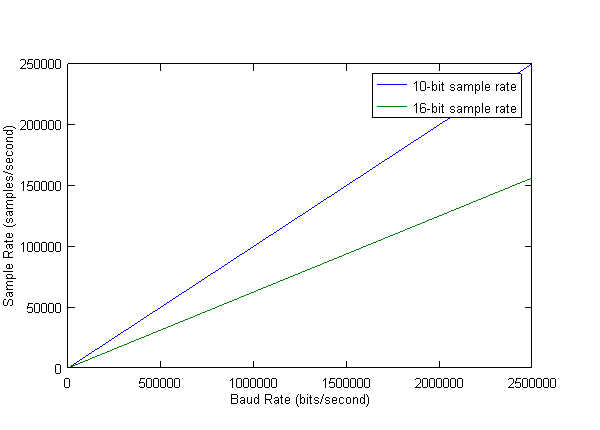
\includegraphics[width=3in]{baud_rate.png}
\label{fig:baud rates and sample}
\end{figure}


